


${}^{23}\mathrm{Ne}$ is unstable.  Over time it converts to ${}^{23}\mathrm{Na}$. Among the products emitted during its decay are photons and these are observed at energies of 
%awk 'BEGIN{g=0;e1=0.440;e2=2.076;e3=2.982; print e1-g, e3-e2,e2-e1,e2-g,e3-e1,e3-g}'
$\gamma_1=0.440~\mathrm{MeV}$, $\gamma_2=0.906~\mathrm{MeV}$, $\gamma_3=1.636~\mathrm{MeV}$, $\gamma_4=2.076~\mathrm{MeV}$, $\gamma_5=2.542~\mathrm{MeV}$ and $\gamma_6=2.982~\mathrm{MeV}$.
\begin{allparts}
\part
By what nuclear process(es) does  ${}^{23}\mathrm{Ne}$ decay to ${}^{23}\mathrm{Na}$ ?\marks{2}


\ANS{

We want the candidates to explain that the neon is initially \textbf{beta} decaying to (possibly though not necessarily) excited states of sodium, and that the excited states are then decaying to the ground state through gamma radiation.  I.e., they need to explain that the diagonal transitions are beta and the vertical transitions are the photons.

}
\part
How many energy-level schemes of the form shown below are compatible with the  gamma ray energy spectrum reported?  \shorthint{You should find more than one.}  Draw an energy-level diagram for each scheme that you find, making sure to label on it: (i) which $\gamma_i$ corresponds to which transition, and (ii) the  %numerical 
values taken by the excitation energies $E_1$, $E_2$ and $E_3$.\marks{3}

\begin{center}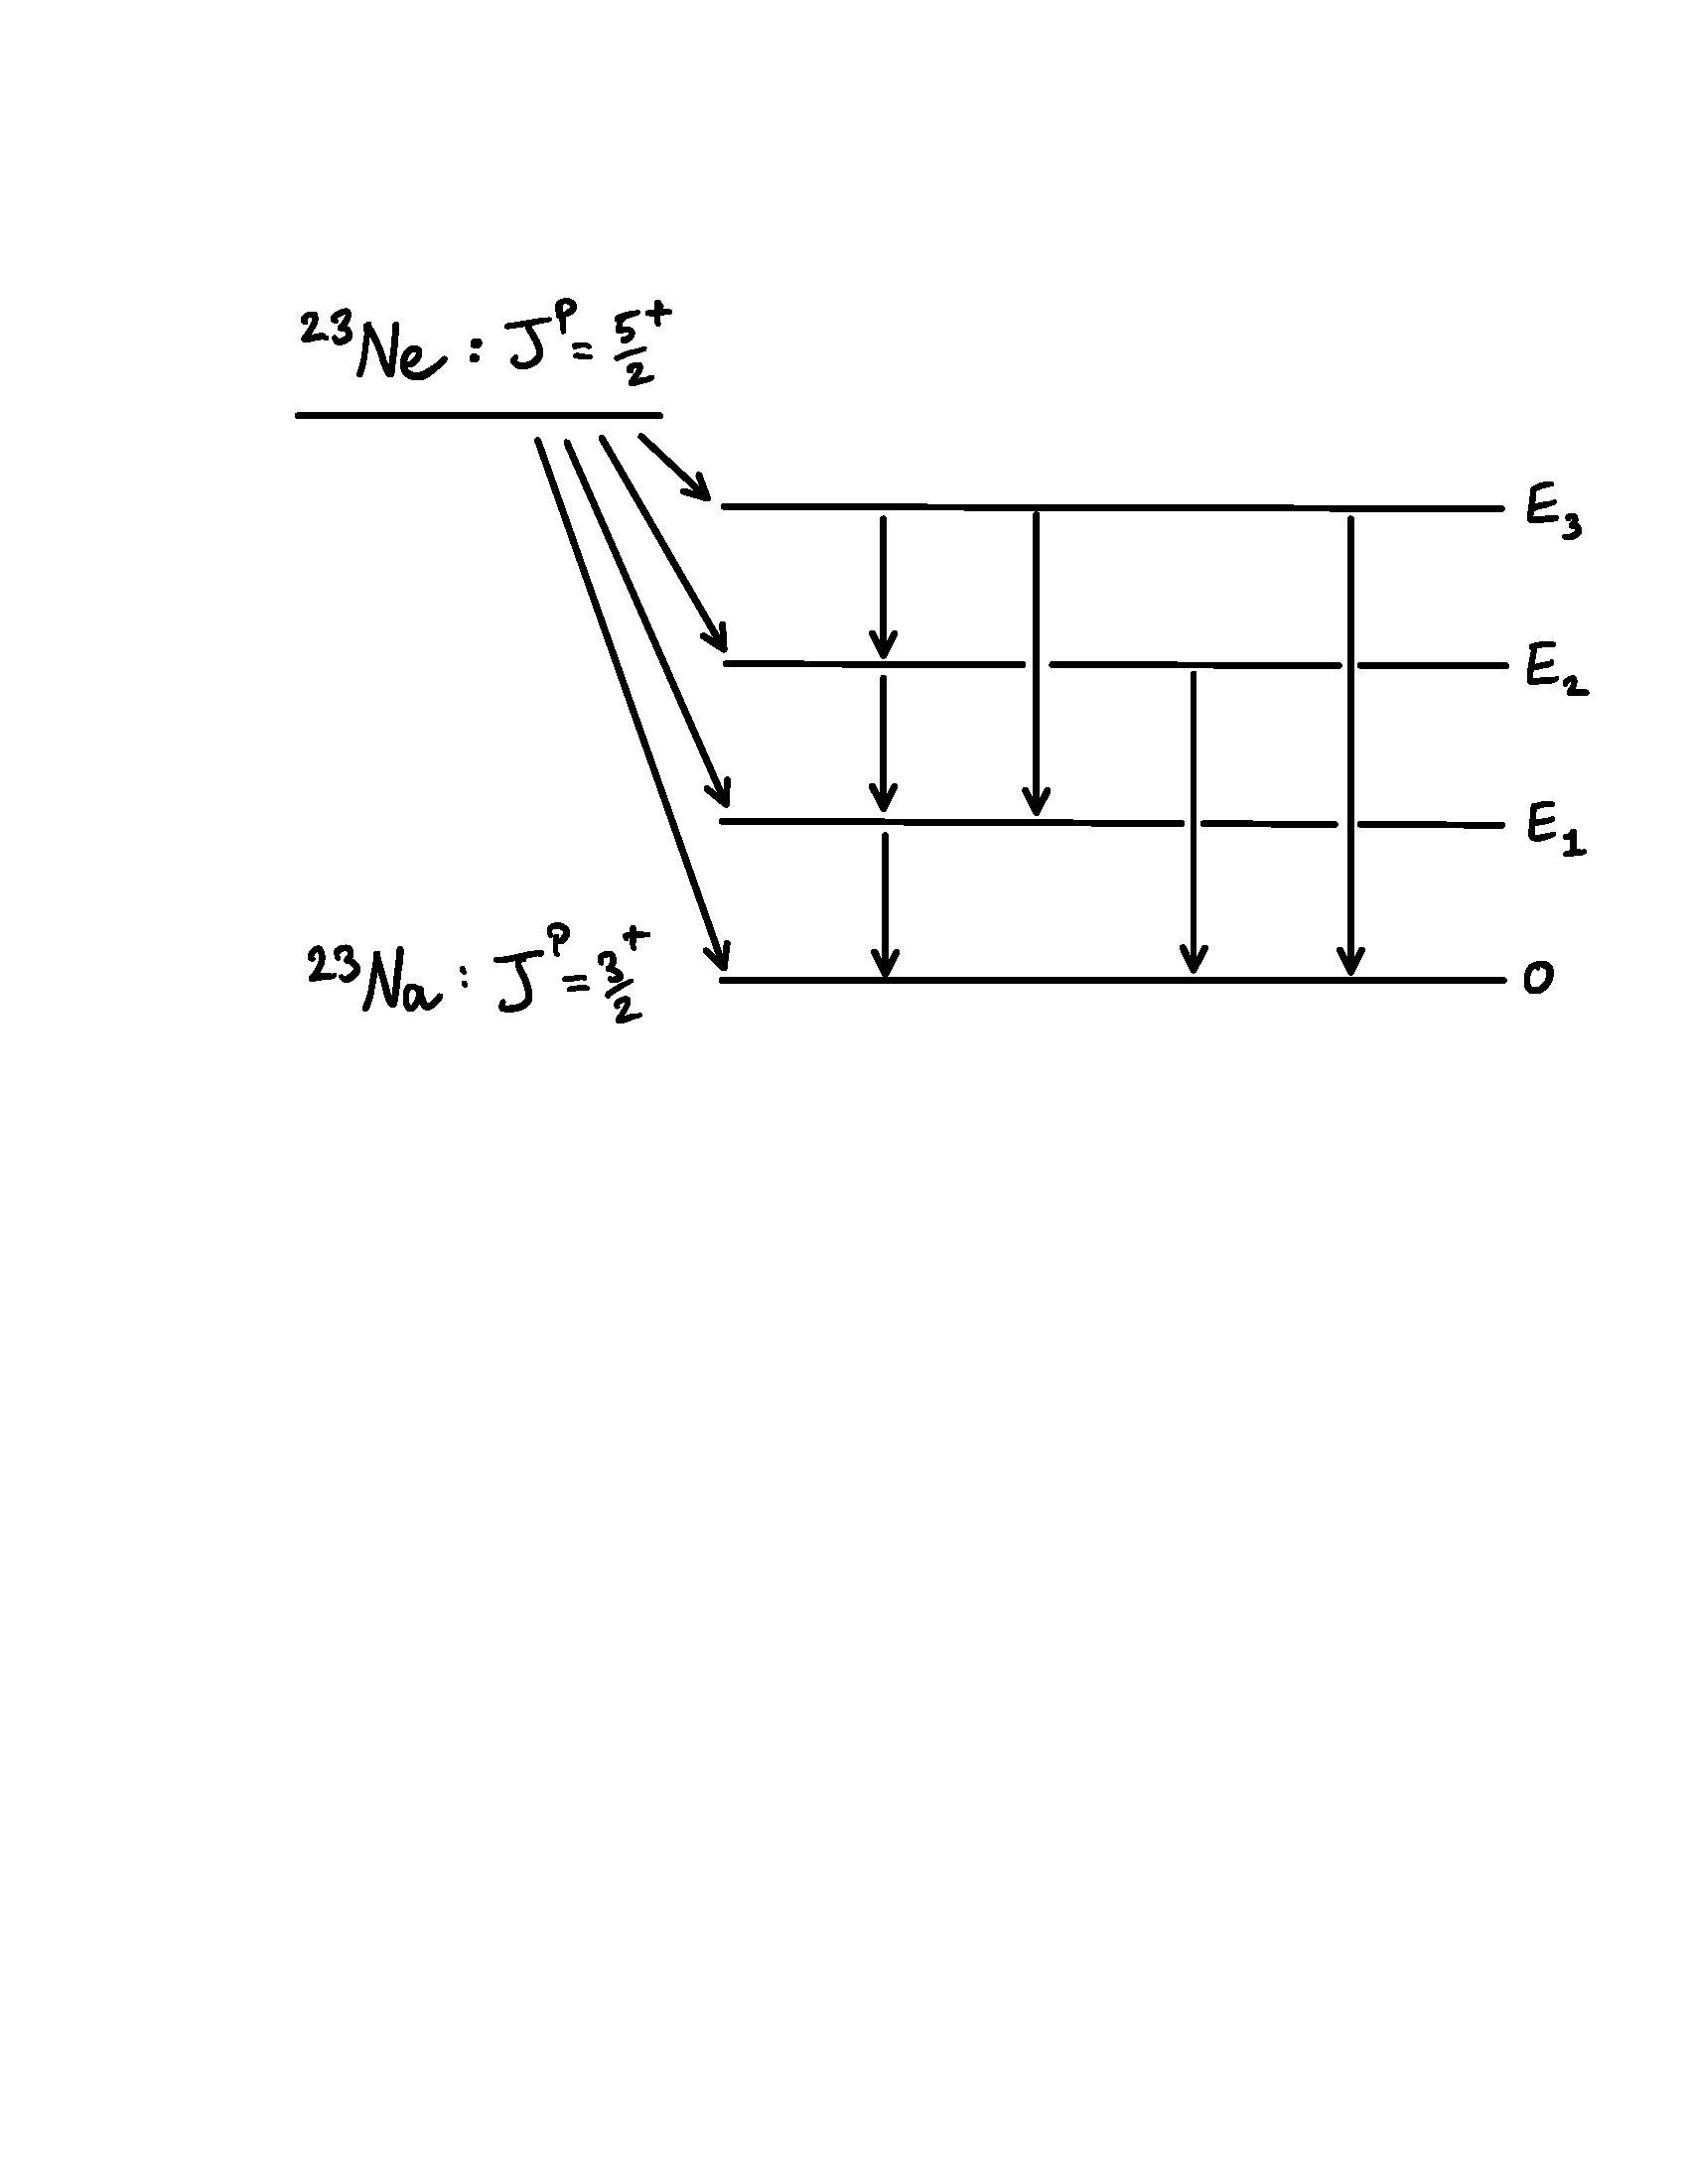
\includegraphics[width=0.65\textwidth]{Images/23Na_energy_levels_ipad.pdf}\end{center}

\ANS{

Any scheme can be inverted to produce a second scheme since $|E_i-E_j| = |E_j-E_i|$. There is only one fundamental four-level scheme that fits the data. We call its non-inverted and inverted variants `Scheme A' and `Scheme B'.  They look like this:


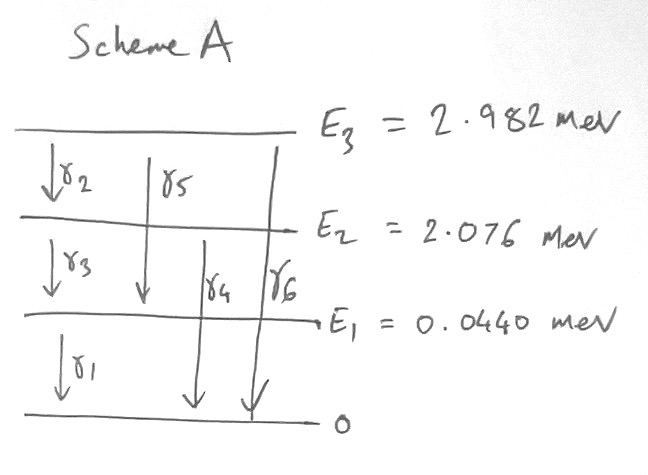
\includegraphics[width=0.7\textwidth]{Images/Scheme_A.jpeg}
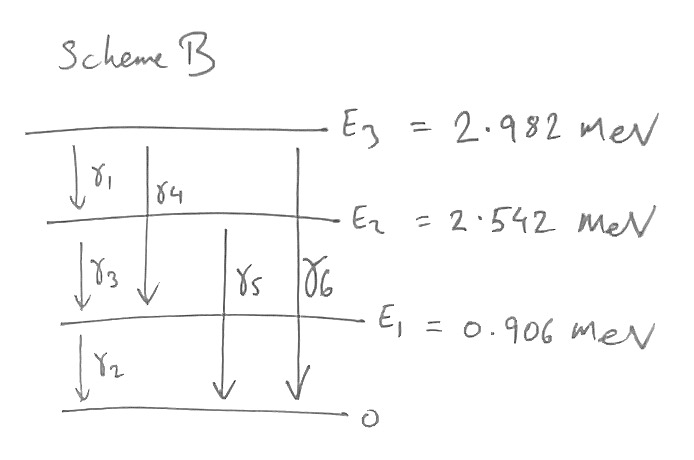
\includegraphics[width=0.7\textwidth]{Images/Scheme_B.jpeg}

}
\end{allparts}
%awk 'BEGIN{g=0;e1=0.440;e2=2.076;e3=2.982; print 1,e1-g, 2,e3-e2,3,e2-e1,   4,e2-g,   5,e3-e1,   6,e3-g;  print; b3=0.065/100; b2=1.10/100;b1=32/100; b0=1-b1-b2-b3; print b0,b1,b2,b3,":",b0+b1+b2+b3;          b32=0.04/100; b31=41.1/100; b30=1-b32-b31; b21=91.1/100; b20=1-b21;  print b30,b31,b32,":",b30+b31+b32 ;    print b21,b20,":",b21+b20;   b10=1;  r3=b3;  i32=r3*b32; i31=r3*b31; i30=r3*b30;    r2=b2+i32;    i21=r2*b21; i20=r2*b20;    r1=b1+i31+i21;      i10=r1*b10;    r0=b0+i30+i20+i10; print r0," should be 1";     i1=i10; i2=i32; i3=i21; i4=i20; i5=i31; i6=i30;      scale=3000000/0.78 ;  print scale*i1,scale*i2,scale*i3,scale*i4,scale*i5,scale*i6;  print;                  print scale*(i1+i4+i6),"    moo     ",scale*(i1-i3-i5),scale*(i3+i4-i2),scale*(i2+i5+i6); print;print;print;VV1=(i1-i3-i5);VV2=(i3+i4-i2);VV3=(i2+i5+i6);print (1-VV1-VV2-VV3),VV1,VV2,VV3 }'
%1 0.44 2 0.906 3 1.636 4 2.076 5 2.542 6 2.982
%
%0.66835 0.32 0.011 0.00065 : 1
%0.5886 0.411 0.0004 : 1
%0.911 0.089 : 1
%1  should be 1
%1.27034e+06 1 38543.2 3765.47 1027.5 1471.5
%
%1.27558e+06    moo      1.23077e+06 42307.7 2500
%
%
%
%0.66835 0.32 0.011 0.00065


\noindent
Observation of a large sample of  ${}^{23}\mathrm{Ne}$ undergoing complete decay reveals  that the numbers of emitted gamma rays having energies $\gamma_1,\gamma_2,\ldots,\gamma_6$ are (in that order) in the relative ratios $N_1:N_2:\ldots:N_6$ with $N_1=1.27\times 10^6$, $N_2=1.00$, $N_3=3.85\times 10^4$, $N_4=3.77\times10^3$, $N_5=1.03\times10^3$ and $N_6=1.47\times 10^3$.
\begin{allparts}
\part
Which energy-level scheme found in part (b) is the most probable given the gamma ray emission-ratio information just given?  Justify your choice.\marks{2}

\ANS{

Other things being equal, Ne would prefer to decay to Na states which are closer to its ground state than those which are more excited;  on the whole the greater energy drop makes the larger transitions more favourable. [1/2 mark]  The transition with energy $\gamma_1$ has the biggest intensity by far ($N_1\gg  N_i$ for all $i\ne1$).  Scheme B has $\gamma_1$ as a transition between levels 3 and 2, while Scheme A has this as a transition between level 1 and the ground state. Scheme B is impossible, therefore, as there should be at least as many gamma transitions OUT of any given unstable energy level as there are gamma transitions INTO that same level\footnote{Non-gamma (i.e.,~beta) transitions directly into the second Na level from Ne would account for the rest needed to balance the INs with the OUTs for level 2.} [1 mark] ... yet $N_3+N_5$ (which is proportional to transitions OUT of level 2 in Scheme B) does not equal or exceed $N_1$ (which is proportional to gamma transitions INTO state 2). Scheme A is therefore the correct one. [1/2 mark]

}

\part
For the most-probable scheme identified in (c) above, and denoting the branching ratios of ${}^{23}\mathrm{Ne}$ to the $0^\textrm{th}$, $1^\textrm{st}$, $2^\textrm{nd}$ and $3^\textrm{rd}$ excited states of ${}^{23}\mathrm{Na}$ by the symbols $\Gamma_0$, $\Gamma_1$, $\Gamma_2$ and $\Gamma_3$  respectively:
\begin{subparts}
\subpart
write down a simple equation relating $\Gamma_0$, $\Gamma_1$, $\Gamma_2$ and $\Gamma_3$; \marks{2}
\subpart
write down additional formulae relating $\Gamma_1$, $\Gamma_2$ and $\Gamma_3$ to the symbols $N_1,\ldots,N_6$ and $\Gamma_0$ so that you may: \marks{8}
\subpart
solve all the equations above simultaneously to determine the numerical values of $\Gamma_1$, $\Gamma_2$ and $\Gamma_3$ under the assumption that $\Gamma_0 =67$\%.\marks{2}
\end{subparts}
%\shorthint{You should avoid substituting numerical values into equations, even the value of $\Gamma_0$, until the end of any calculation.}%\marks{12}


\ANS{

The first part is simple. By definition:
$\Gamma_0+\Gamma_1+\Gamma_2+\Gamma_3=1$.

The second and third parts take more time:

The quantities $N_i$ specify \textbf{relative} intensities (or \textbf{relative} rates) but do not fix \textbf{absolute} ones.  Use this freedom, therefore, to work in an imaginary scenario in which the absolute rate of production of 23Ne is one nucleus per unit time.  In this scenario, the numerical values for the branching ratios $\Gamma_i$ are also the rates for the production (via beta decay) of the $i^\textrm{th}$ excited state.  Furthermore, denoting by $\rho_i$ the rate of production of $\gamma_i$, we will have $\rho_i = k N_i$ for some (unknown) constant $k$ which is independent of $i$.  With that notation we are in a position to write down an equation which expresses the idea that the number of decays INTO level 3 must be the same as the number of decays OUT OF level 3:
$$ \Gamma_3 = \rho_2+\rho_5+\rho_6.$$
Similarly, the equation which expresses the idea that the number of decays INTO level 2 must be the same as the number of decays OUT OF level 2 is:
$$ \Gamma_2 + \rho_2 = \rho_3+\rho_4$$
while that balancing inflows and outflows for level 1 is:
$$\Gamma_1+\rho_3+\rho_5 = \rho_1.$$
Finally the statement that `all the neon ends up in the ground state' is
$$\Gamma_0+\rho_1+\rho_4+\rho_6=1.$$

\noindent[Aside: adding the four equations above and then cancelling the expression  $\sum_{i=1}^6 \rho_i$ which appears on both sides  reproduces the first equation we wrote down: $$\Gamma_0+\Gamma_1+\Gamma_2+\Gamma_3=1.$$ 
We do not need to notice this fact, but it is a sensible consistency check!]


\noindent The vector of branching ratios
$[\Gamma_0,\Gamma_1 , \Gamma_2 , \Gamma_3]$ is therefore
\begin{align}
[\Gamma_0,\ \Gamma_1,\  \Gamma_2 ,\  \Gamma_3]
&=
[1-(\Gamma_1+\Gamma_2+\Gamma_3),
\Gamma_1 , \Gamma_2 , \Gamma_3]\nonumber
\\
&=
[ 1-(\rho_1+\rho_4+\rho_6)
,\ 
(\rho_1-\rho_3-\rho_5)
,\ 
(\rho_3+\rho_4-\rho_2)
,\ 
(\rho_2+\rho_5+\rho_6)
]\nonumber
\\
&=
[ 1 -(N_1+N_4+N_6)k
,\ 
(N_1-N_3-N_5)k
,\ 
(N_3+N_4-N_2)k
,\ 
(N_2+N_5+N_6)k
]\nonumber
%\\
%&=
%k[\frac 1 k - 1.27558\times %10^6,(N_1-N_3-N_5)
%,
%(N_3+N_4-N_2)
%,
%(N_2+N_5+N_6)].\nonumber
%\\
%&=
%k[\frac 1 k - 1.27558e+06, 1.23077\times10^6 , 42307.7 , 2500].\nonumber
.
\end{align}
In particular: $$\Gamma_0=1-(N_1+N_4+N_6)k$$ and so \begin{align}k= \frac{1-\Gamma_0}{N_1+N_4+N_6}.\label{eq:thingfork}\end{align}
\hide{which means that 
\begin{align}
[\Gamma_0,\Gamma_1 , \Gamma_2 , \Gamma_3]
&=
[\Gamma_0
,
\frac{N_1-N_3-N_5}{N_1+N_4+N_6}(1-\Gamma_0)
,
\frac{N_3+N_4-N_2}{N_1+N_4+N_6}(1-\Gamma_0)
,
\frac{N_2+N_5+N_6}{N_1+N_4+N_6}(1-\Gamma_0)
].\nonumber
\end{align}
}

\noindent The question gives values of $N_i$ from which we can compute that:
\begin{align}
N_1-N_3-N_5&\approx 1.23\times10^6
\\
N_3+N_4-N_2&\approx 42300 
\\
N_2+N_5+N_6&\approx 2501.
\end{align}
The question also tells us $\Gamma_0=0.67$ and so \eqref{eq:thingfork} implies:
\begin{align}
k
&=
\frac{1-0.67}{1.27\times 10^6+3.77\times10^3+1.47\times 10^3}\nonumber
\\
&=\frac{0.33}{1.275240\times 10^6}\nonumber
\\
&\approx 2.59\times 10^{-7}\nonumber
\end{align}
and hence putting the above together:
\begin{align}
[\Gamma_0,\Gamma_1 , \Gamma_2 , \Gamma_3]
&\approx
[0.67,
( 1.23\cdot 10^6)\cdot (2.59\cdot 10^{-7}), 42300 \cdot (2.59\cdot 10^{-7}), 2501\cdot (2.59\cdot 10^{-7})
]\nonumber
\\
&\approx
[0.670,
0.318, 0.0109, 0.00065]\nonumber
\\
&=
[67.0\%, 31.8\%, 1.09\%, 0.065\%]. \nonumber
\end{align}
This question is based on Fig 14 in  \url{http://dx.doi.org/10.1140/epja/i2018-12526-2} and was designed to give the branching ratios it reports.
}


\end{allparts}
\hide{
The ground state of ${}^{23}\mathrm{Na}$ is known to have $J^P={\frac 3 2}^+$. Suppose that transitions $\gamma_2$ and $\gamma_4$ are known to be E2 (electric quadrupoles), while all the other transitions are M1/E2 (magnetic dipole or electric quadrupole).

\begin{allparts}
\part
What are the spins and parities of the excited states of ${}^{23}$Na which are produced in decays of ${}^{23}$Ne ?\marks{4}

\answer

At this point we have 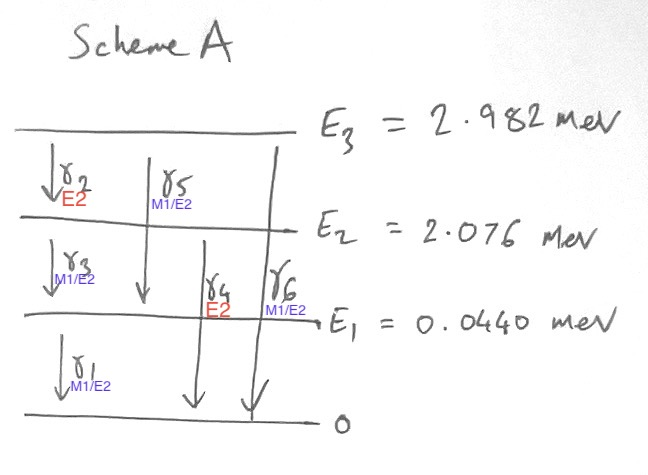
\includegraphics[width=0.7\textwidth]{Images/Scheme_A_with_poles.jpeg}

\begin{itemize}
\item
Neither E2 nor M1 induce a parity change, therefore all the excited states we are looking at have parity $P=+$ just like the ground state.
\item
The presence of an E2 transition ($\gamma_4$) from level-2 to ground together with the absence of an M1 for the same gap means that level-2 has a spin that is two units away from the ground state.  This fixes level-2 as $J^P={\frac 7 2}^+$
\item
The presence of an M1 transition between level-1 and EVERY OTHER STATE means that level-1 is at most one unit of spin away from every other level. But with other levels already at ${\frac 3 2}^+$ and ${\frac 7 2}^+$, that leaves only one possibility: level-1 has $J^P={\frac 5 2}^+$.
\item
The presence of an E2 transition ($\gamma_2$) from level-3 to level-2 together with the absence of an M1 for the same gap means that level-3 has a spin that is two units away from level-2.  This suggests level-3 is either  ${\frac 3 2}^+$ or ${\frac {11} 2}^+$.  The latter option is excluded by the M1 transition ($\gamma_5$) from level-3 to level-1.  Therefore level-3 is $J^P={\frac 3 2}^+$.
\end{itemize}
In summary, we have (as reproduced from Fig 14 of \url{http://dx.doi.org/10.1140/epja/i2018-12526-2} )

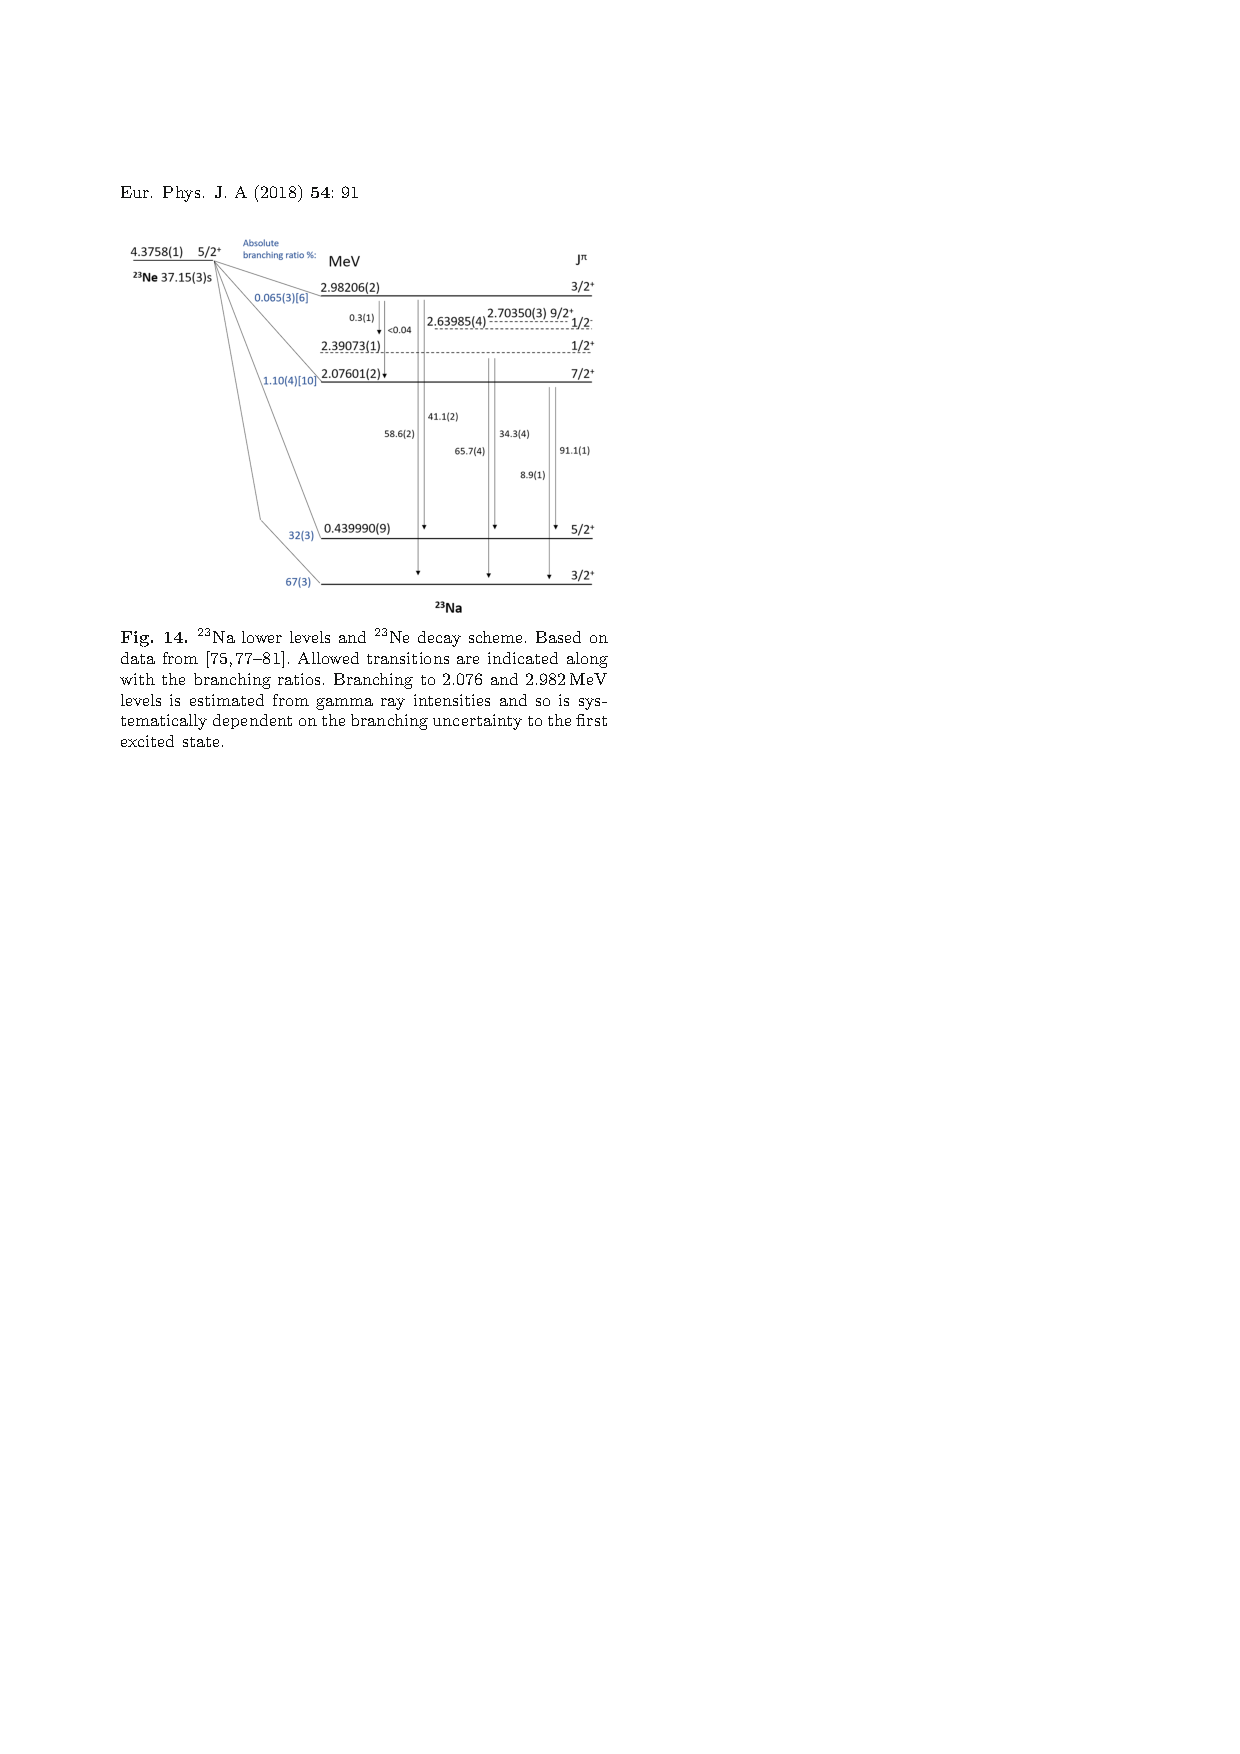
\includegraphics[width=0.8\textwidth]{Images/23Na_spectrum_from_paper.pdf}

\endanswer

\end{allparts}
}